Пусть на вход подаётся последовательность символов латинского алфавита. Рассмотрим работу конвейера для шифрования этих данных.

\section{Используемые алгоритмы шифрования}

\subsection{Алгоритм, в основе которого лежит операция XOR}
\qquadНа вход подаётся строка и ключ. Этот алгоритм шифрования разбит на две части: сначала прозводится операция XOR каждой буквы строки с первой буквой ключа, зачем с каждой третьей буквой дополнительно производится та же операция, только уже со второй буквой ключа (при условии, что длина ключа больше 1).\\

\textbf{Схема} алгоритма представлена на Рис.\ref{fig1:image}.\\
\begin{figure}[h]
	\begin{center}
		{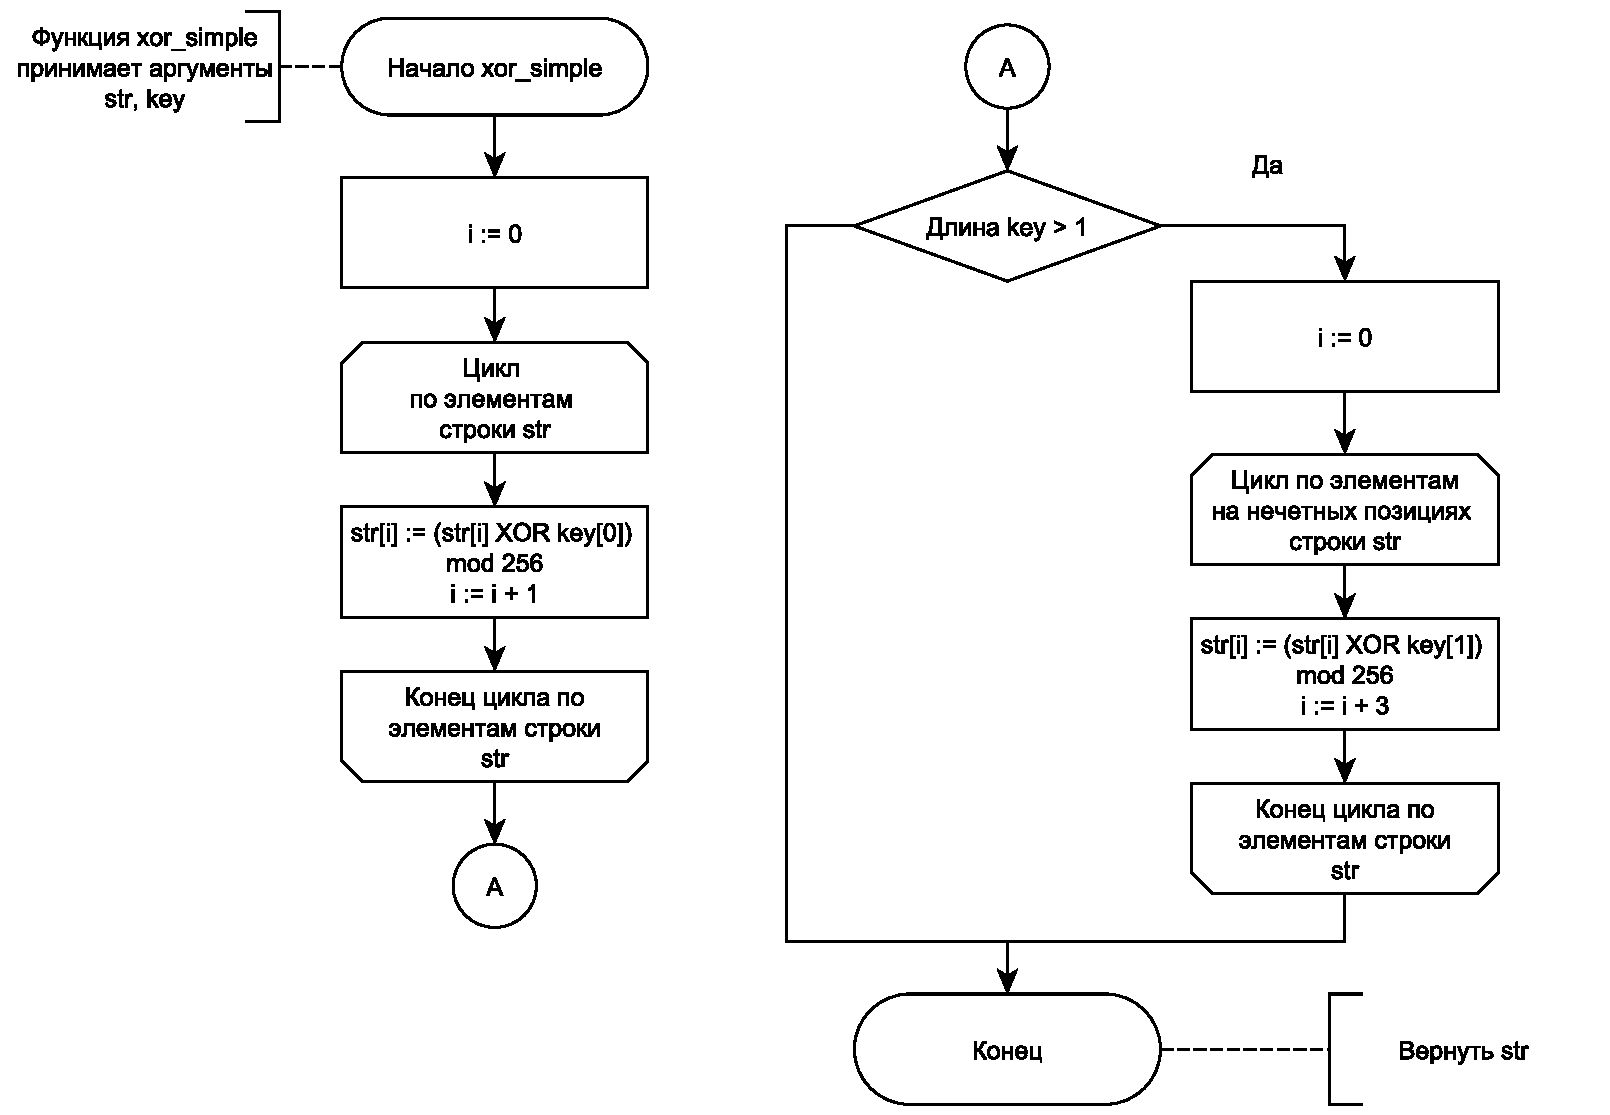
\includegraphics[scale = 0.65]{schemes/xor}}
		\caption{Алгоритм, в основе которого лежит операция XOR}
		\label{fig1:image}
	\end{center}
\end{figure}

\newpage
 
\subsection{Шифр Виженера}
\qquadНа вход тоже подаётся строка и ключ. Реализовывается проход по всем элементам строки, и согласно формуле \ref{formula1}, код текущего символа складывается с кодом соответствующего ему символа ключа, и затем по полученному коду определяется сам символ.\\

Если ключ короче исходной строки, то он используется циклически, т.е. после последнего символа ключа вновь происходит переход к первому.\\

\textbf{Схема} алгоритма представлена на Рис.\ref{fig2:image}.\\
\begin{figure}[h]
	\begin{center}
		{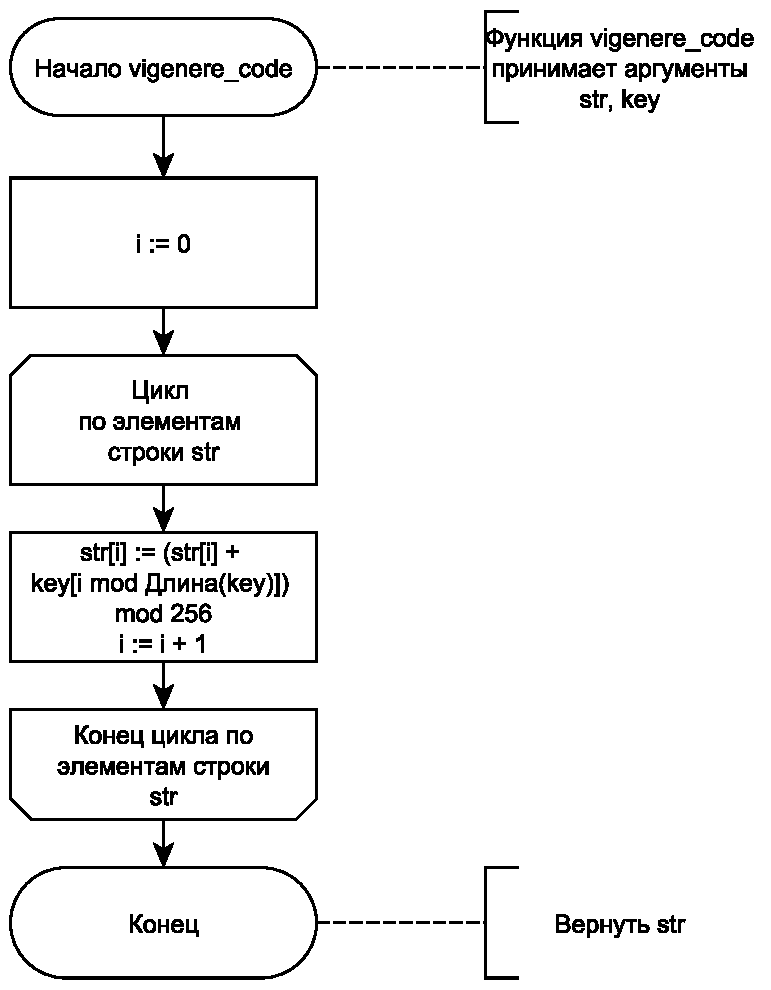
\includegraphics[scale = 0.65]{schemes/vigenere}}
		\caption{Шифр Виженера}
		\label{fig2:image}
	\end{center}
\end{figure}

\newpage

\subsection{Транспозиция}
\qquadВ этом алгоритме используется только символьная строка. В рассматриваемом методе используется двойная перестановка. Сначала переставляются элементы попарно, а затем все элементы первой половины строки, стоящие на нечетных позициях, меняются местами с симметричными относительно середины строки элементами.\\

\textbf{Схема} алгоритма представлена на Рис.\ref{fig3:image}.\\
\begin{figure}[h]
	\begin{center}
		{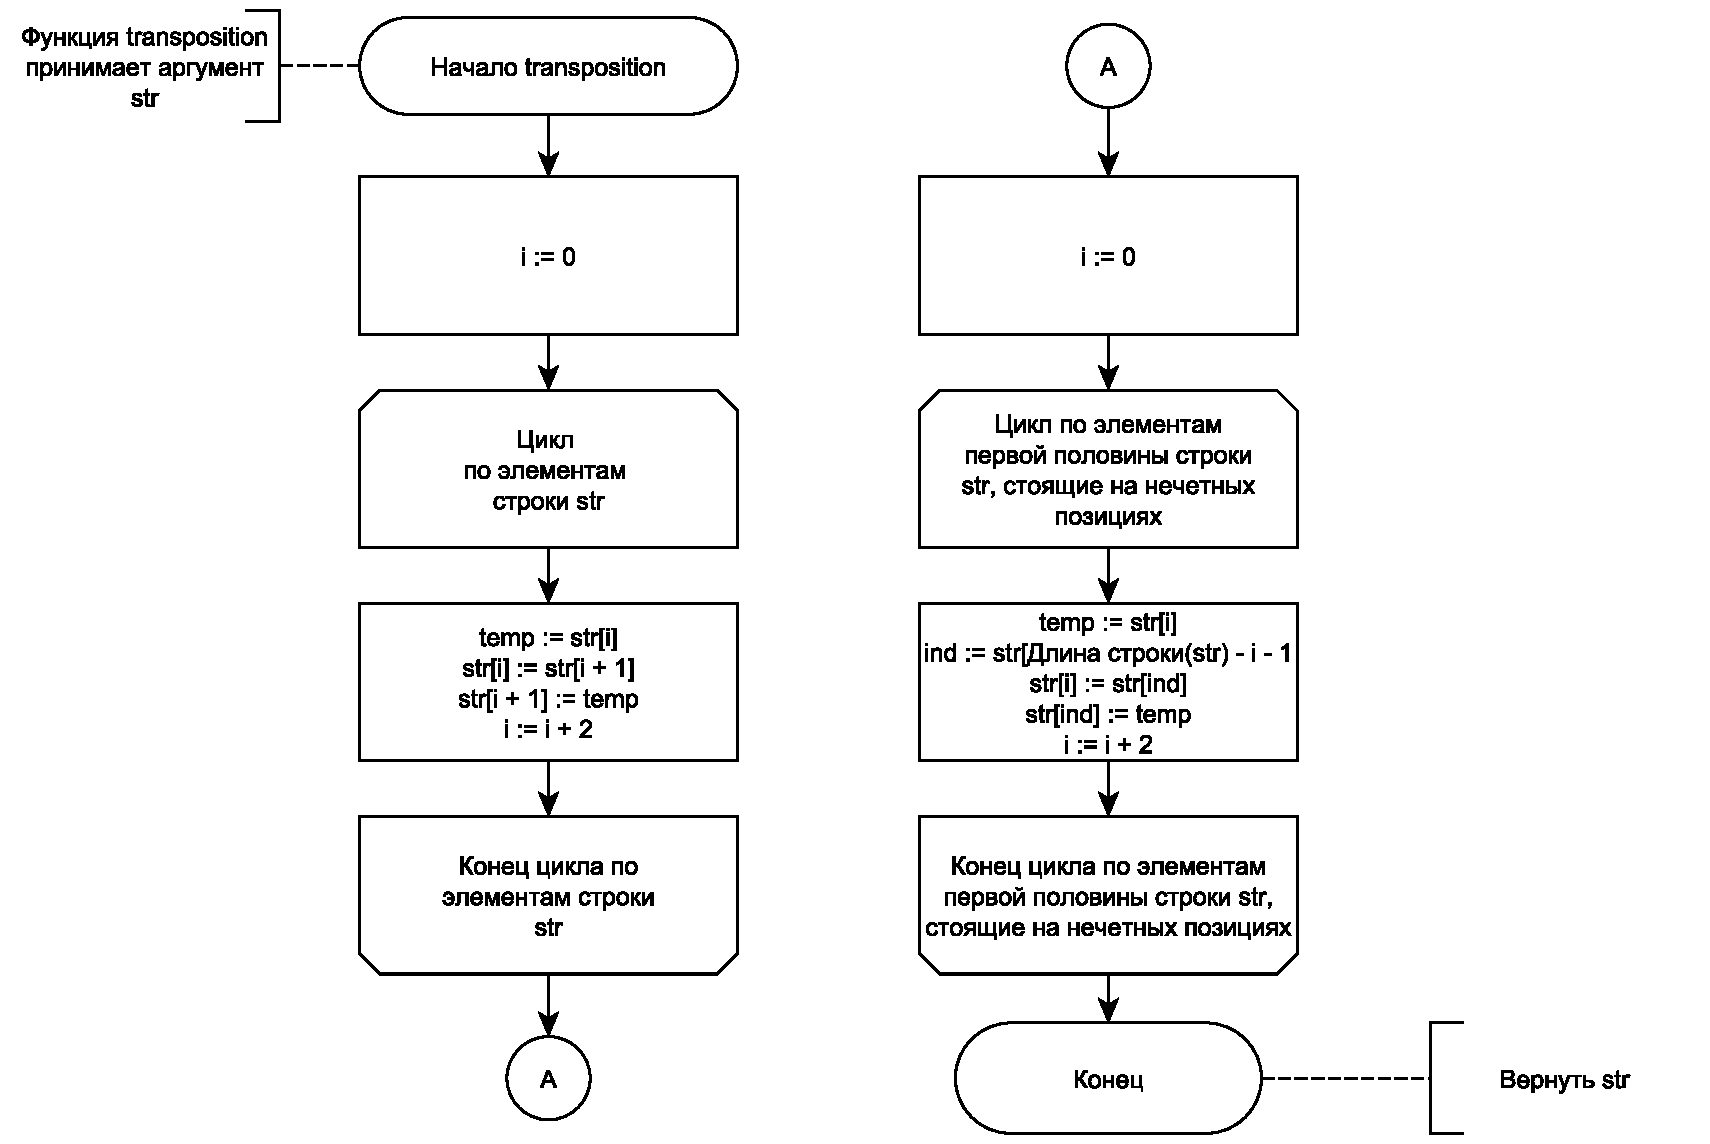
\includegraphics[scale = 0.65]{schemes/trans}}
		\caption{Транспозиция}
		\label{fig3:image}
	\end{center}
\end{figure}

\newpage

\section{Организация работы конвейера}
\qquadКак упоминалось выше, рассматриваемый конвейер состоит из трёх лент, каждая из которых обрабатывается своим потоком. Перед тем, как поступить на какую-либо ленту задача попадает в очередь и ожидает дальнейшей обработки. \\

Первая очередь заполняется заранее, число задач указывается пользователем. Если ещё не все задачи обработаны, а очередь на какую-либо стадию обработки пустая, то лента уходит в режим ожидания следующего объекта.\\

Время обработки на лентах примерно одинаковое, и выполняется условие \ref{formula2}.
\begin{equation}\label{formula2}
	t_{processing} >> t_{dispatching}
\end{equation} 

Работа конвейера представлена на \textbf{схемах}: главный поток -- Рис.\ref{fig4:image}, рабочие потоки -- Рис.\ref{fig5:image} (1-ая лента), Рис.\ref{fig6:image} (2-ая лента), Рис.\ref{fig7:image} (3-я лента).\\
\begin{figure}[h]
	\begin{center}
		{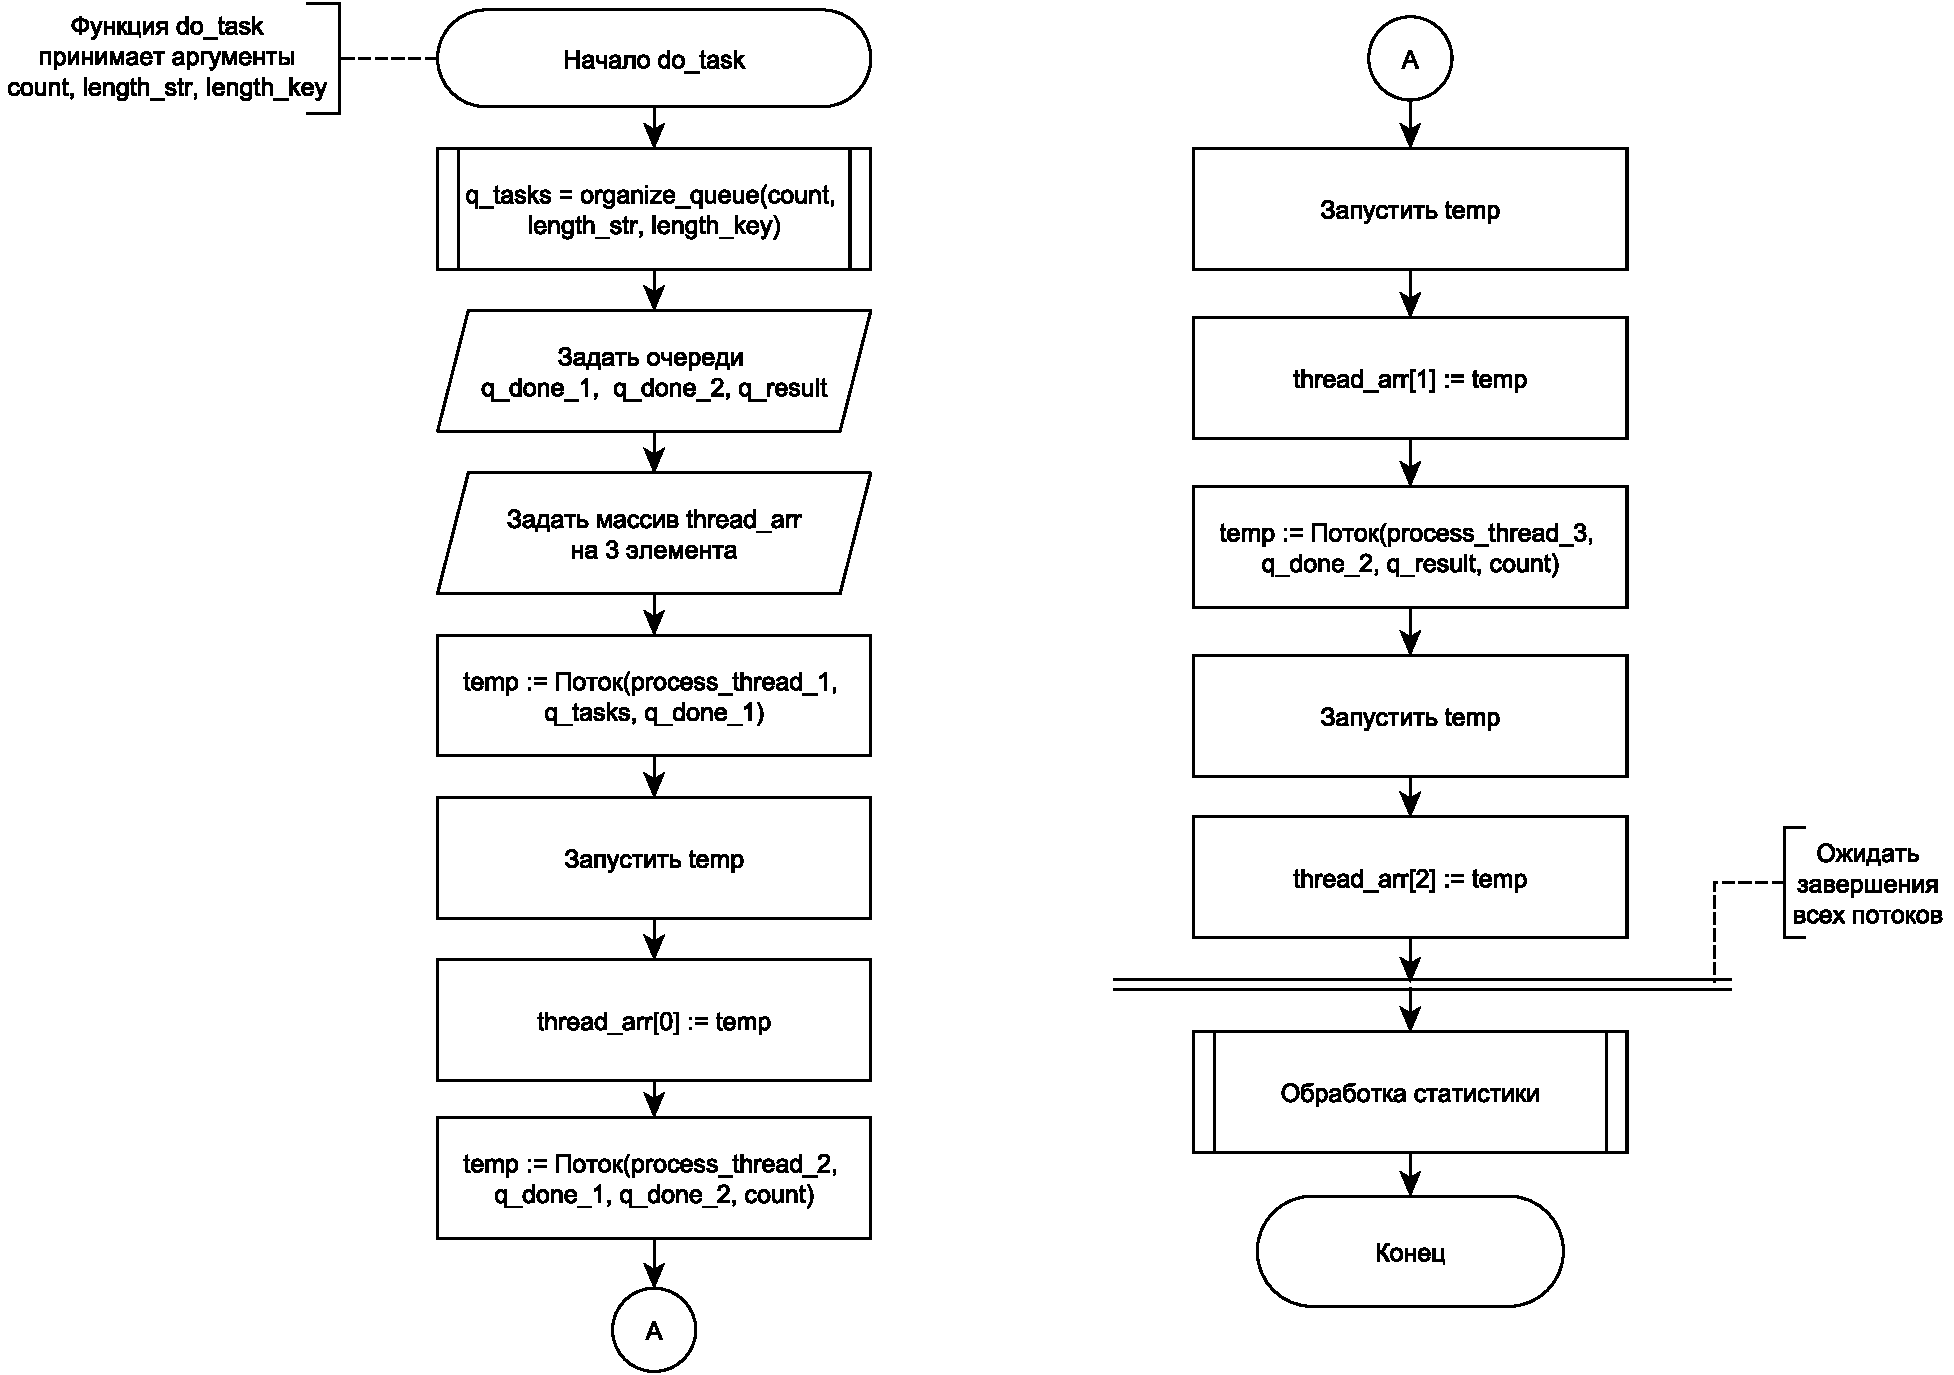
\includegraphics[scale = 0.5]{schemes/conveyor}}
		\caption{Организация работы конвейера. Главный поток}
		\label{fig4:image}
	\end{center}
\end{figure}

\newpage

\begin{figure}[pt!]
	\begin{center}
		{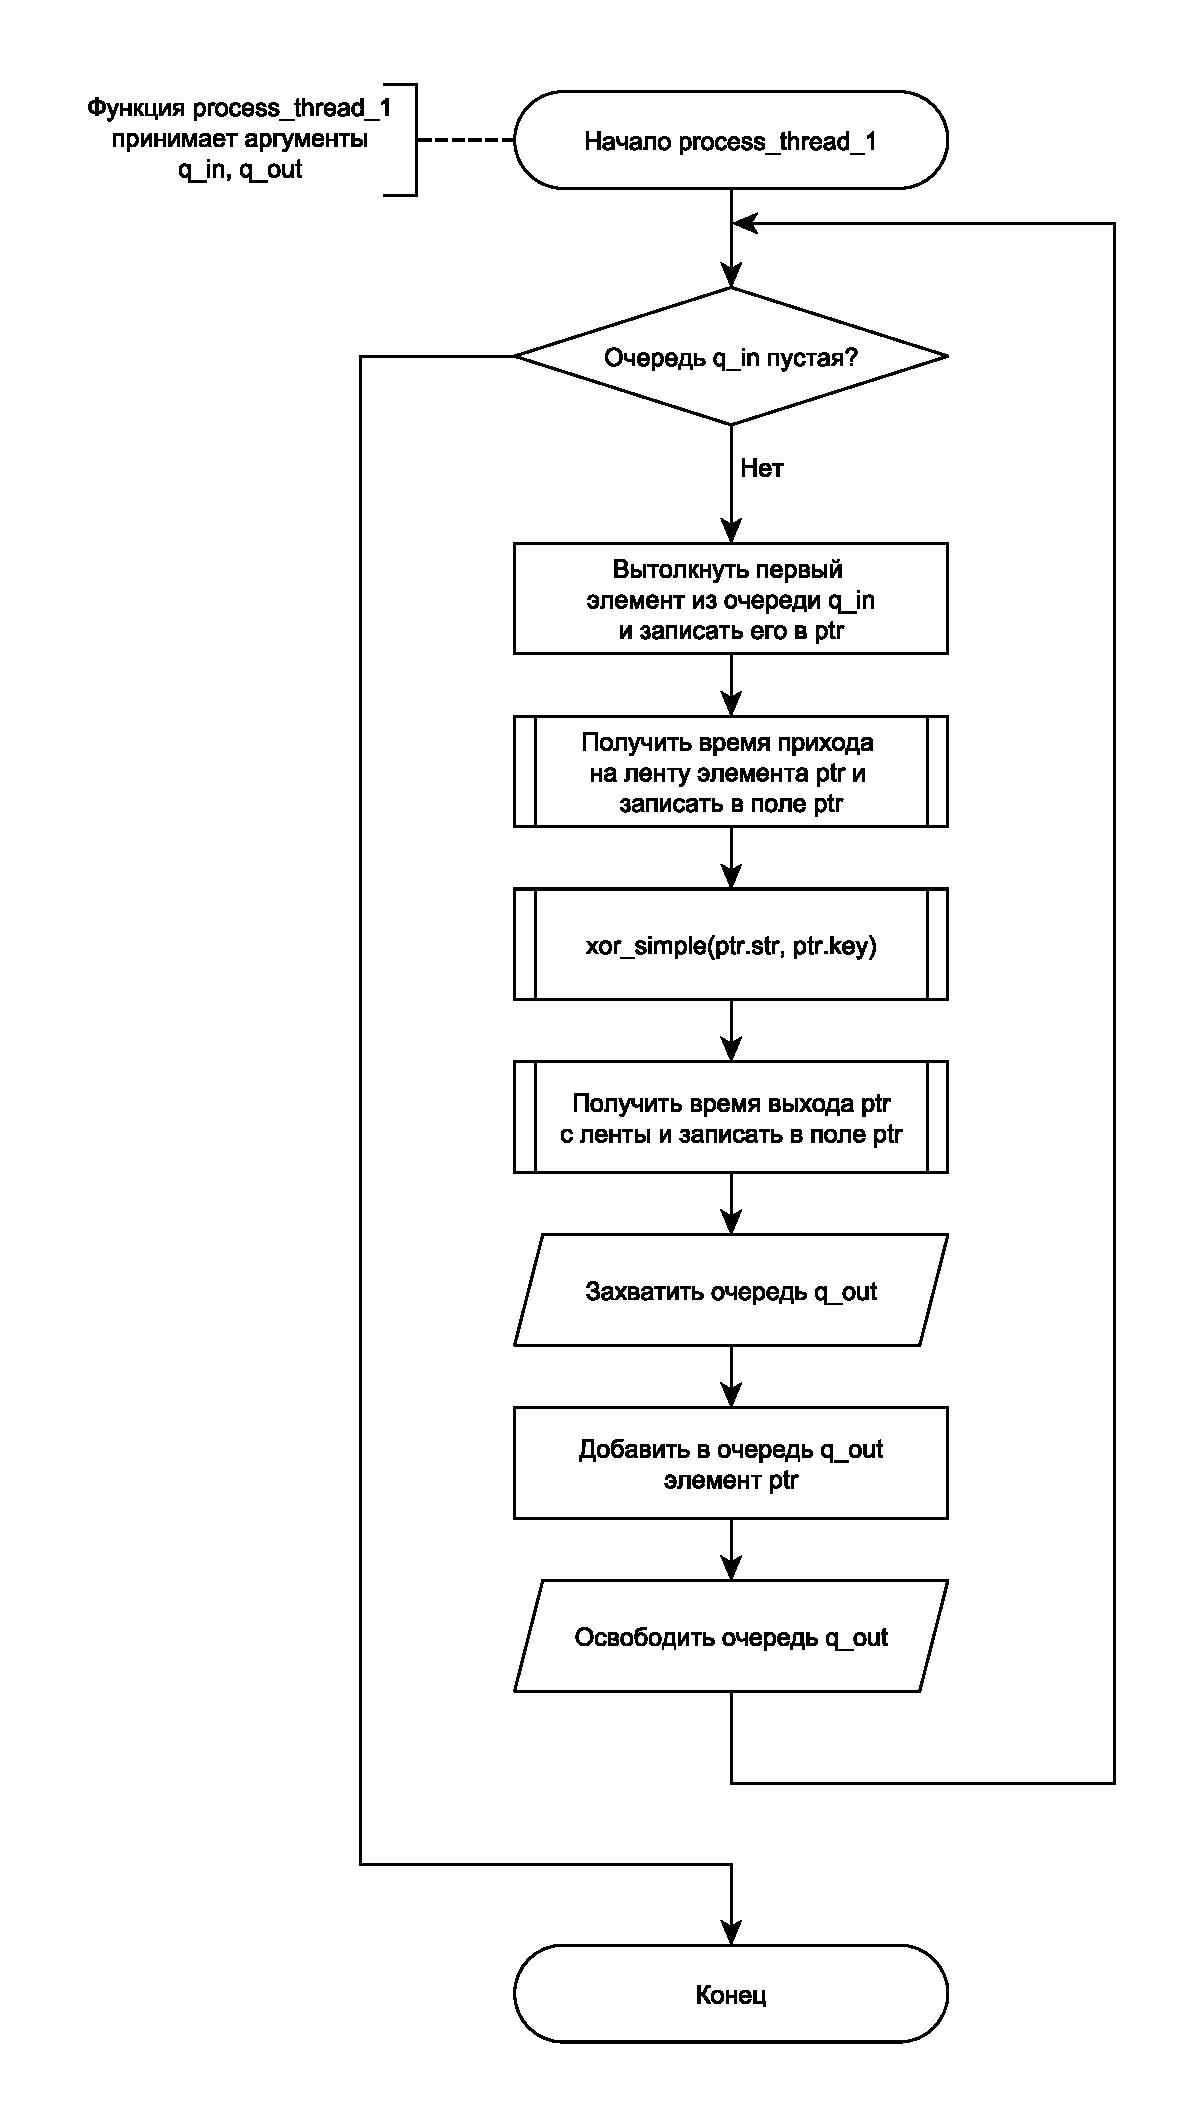
\includegraphics[scale = 0.55]{schemes/line_1}}
		\caption{Организация работы конвейера. Лента 1, рабочий поток}
		\label{fig5:image}
	\end{center}
\end{figure}

\begin{figure}[pt!]
	\begin{center}
		{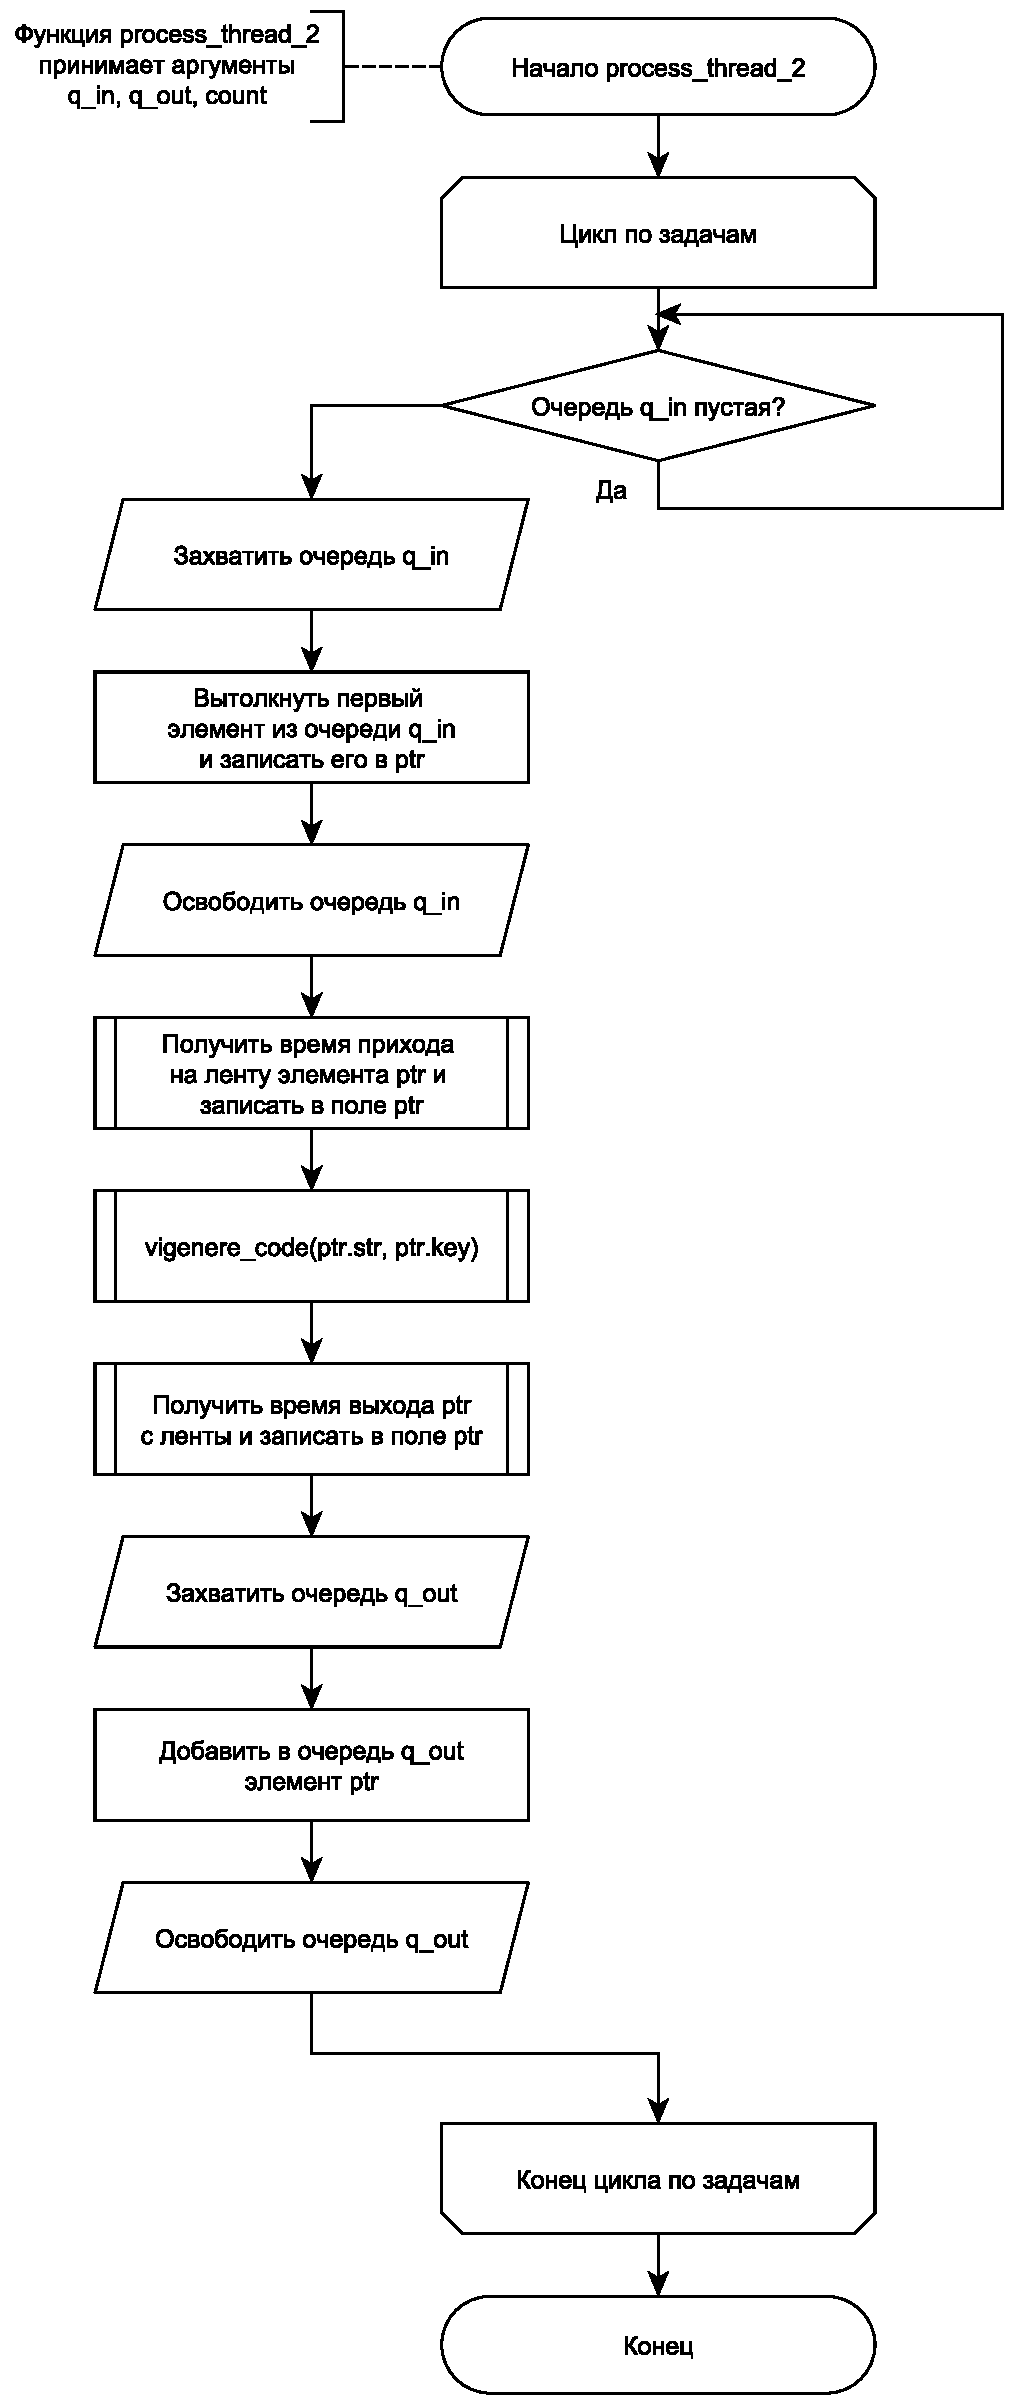
\includegraphics[scale = 0.55]{schemes/line_2}}
		\caption{Организация работы конвейера. Лента 2, рабочий поток}
		\label{fig6:image}
	\end{center}
\end{figure}

\newpage

\begin{figure}[pt!]
	\begin{center}
		{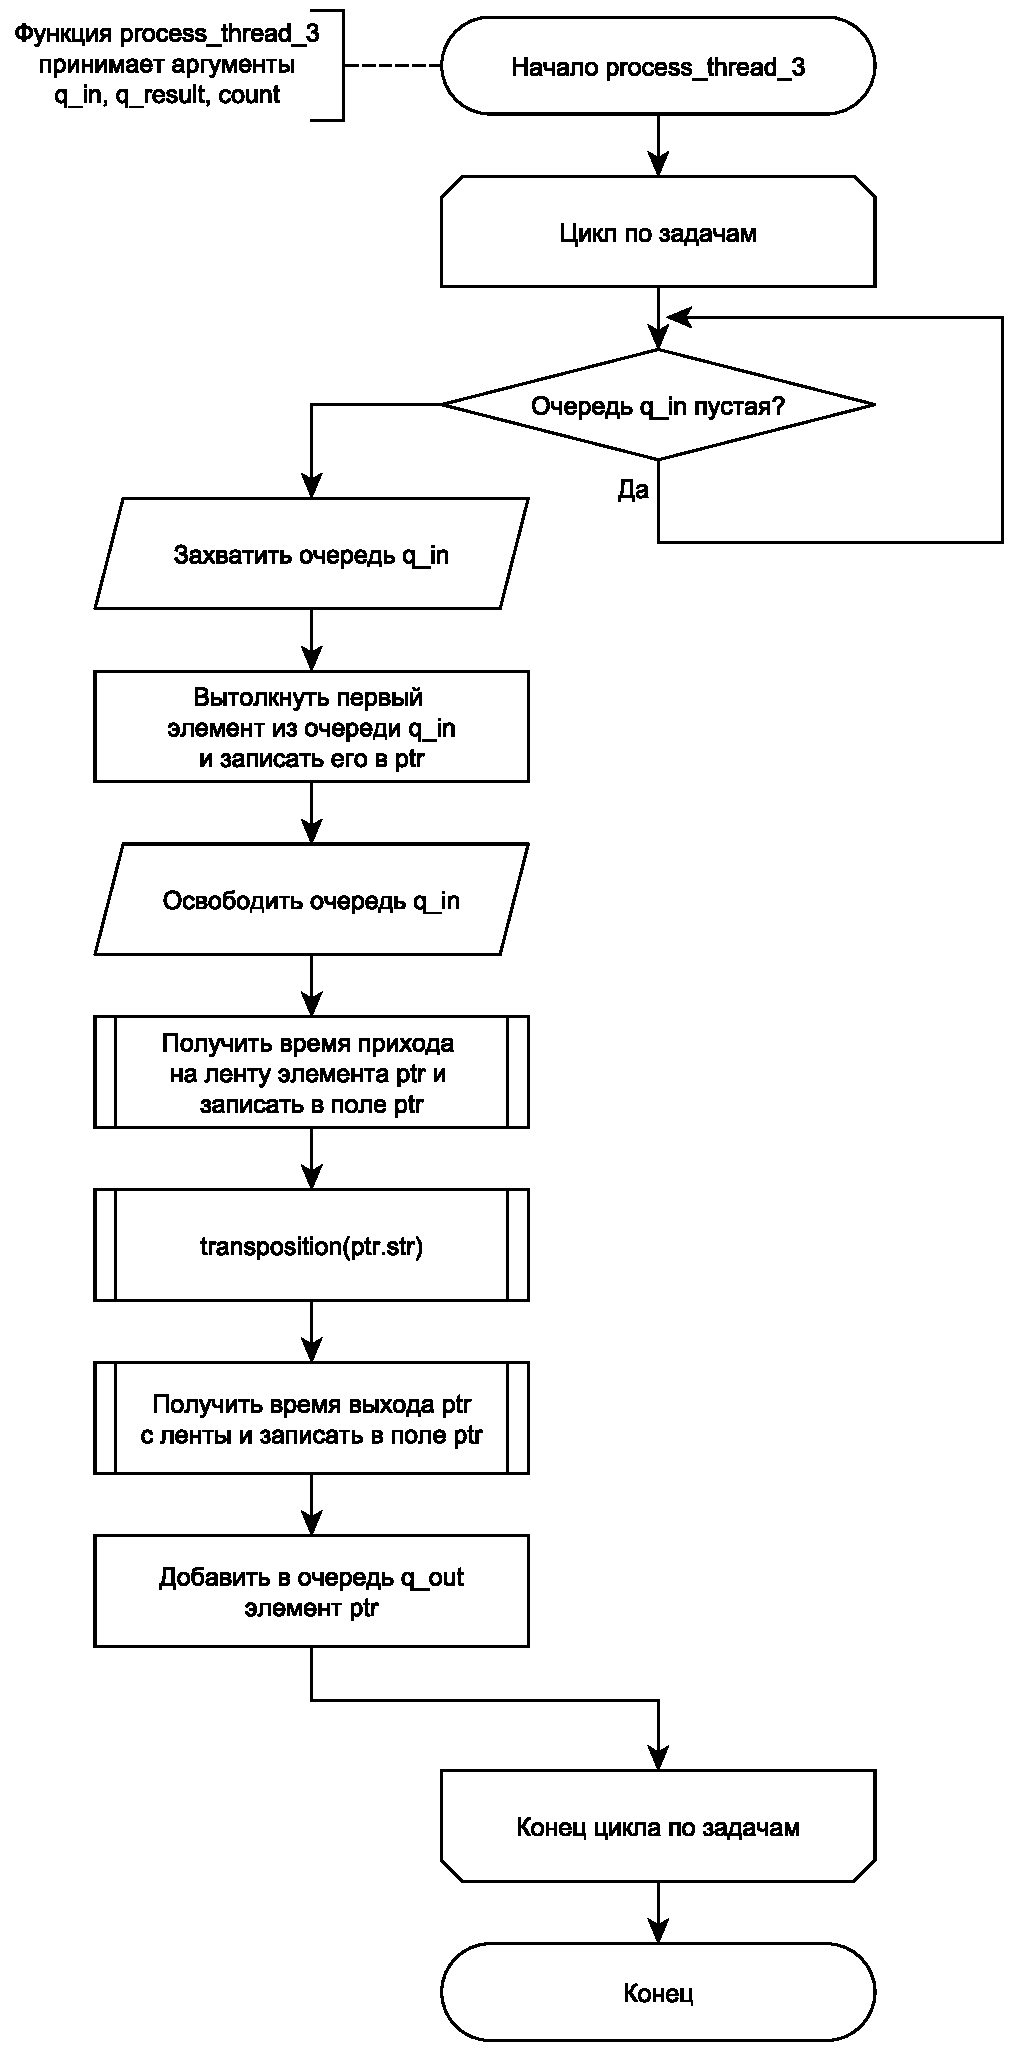
\includegraphics[scale = 0.57]{schemes/line_3}}
		\caption{Организация работы конвейера. Лента 3, рабочий поток}
		\label{fig7:image}
	\end{center}
\end{figure}

\section{Требования к ПО}
\qquadДля корректной работы алгоритмов и проведения тестов необходимо выполнить следующее.
\begin{itemize}
	\item Обеспечить возможность ввода количества задач через консоль.
	\item В случае ввода некорректных данных вывести соответствующее сообщение. Программа не должна аварийно завершаться.
	\item Каждая лента должна работать в своём потоке.
	\item Обеспечить возможность отслеживания времени, когда каждая задача была подана на конкретную ленту конвейера и когда закончилась её обработка.
	\item Реализовать возможность вывода на экран максимальных, минимальных и средних значений времени обработки целой задачи и ожидания в очереди, и итоговое время работы системы.
\end{itemize}

\section{Заготовки тестов}
\qquadПри проверке на корректность работы конвейера необходимо провести следующие тесты:
\begin{itemize}
	\item количество задач меньше 10;
	\item количество задач больше 30.
\end{itemize}

\section*{Вывод}
\addcontentsline{toc}{section}{Вывод}
\qquadВ этом разделе разобраны основные принципы выбранных алгоритмов шифрования, построены схемы. Также описана работа конвейера, его составных частей, приведены соответствующие схемы. Приведены требования к программному обеспечению и написаны заготовки тестов, которые будут использоваться в дальнейшем.
